\chapter{Further work on the model}
\label{secondPhaseOfModelingCyberInsurance} 

In the earlier model, the experienced network effects only arose from their neighbours. I.e. when a node establish a connection the change in utility where only dependent on fixed variables, and non dependent of the rest of the network. In some real world scenarios there is more realistic that a node will be strongly affected by the indirect connections to other nodes as well. Our idea is based on the paper from Jackson and Wolinsky \cite{jackson1996strategic} and a network formation game in \cite{jackson2005survey}. 

\section{The connection game}
The benefits a player receives in this game are calculated as follows. In addition to the benefit from the direct connection, a node will also benefit from "the friends of the friend", and "the friends of the friends of the friend" etc. This is achieved by letting the payoff be calculated relative to the distance between the nodes. $\beta$ is now dependent on the minimum number of hops to the node e.g. the benefit of a direct connection is $\beta$, the benefit of a friend of a friend is $\beta^2$ etc. We want the benefit to decrease with the distance, therefore we need the limitation: $0<\beta<1$. 
\begin{figure}[h]
\centering
  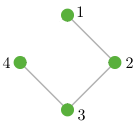
\includegraphics[width=0.2\linewidth]{../Figures/connectionGame.png}
  \caption{\label{fig:connectionGame} Four nodes interconnected with each other.}
\end{figure}
\subparagraph{Example}Lets consider the network shown in \ref{fig:connectionGame}. Node 1 and node 4, in the network will receive a benefit of $\beta+\beta^{2}+\beta^{3}$ by being connected with node 2 and 3. $\beta^{2}+\beta^{3}$ represents the indirect benefits from node 3 and 4. Node 2 and 3 receives a benefit of $\beta+\beta+\beta^{2}$. For this network to make sense, it is important to also include some cost of having direct connections, or else the rational thing would be to establish a link with everyone. This is done as in earlier models, every node pay a cost for direct connections, but no cost for indirect connections. Thus the total payoff for a node is:

\begin{equation}
\sum_{j\neq i}^{} \beta_{ij}^{d(ij)} - \sum_{j:ij\in g}^{} {c}_{ij}, 
\label{eq:connecetionGame}
\end{equation}

where $d(ij)$ represents the shortest path between node $i $ and node $j $, and ${c}_{ij}$ represents node i's cost of establishing a link between the two nodes. To simplify the model we choose a symmetric connection process where $\beta$ and $c$ is set to a fixed global value. 

In the paper \cite{jackson1996strategic}, they analyze two different networks outcomes, one with the focus on efficiency and the other on stability. An efficient network means ending up with a network where the sum of every nodes payoff is maximized. The optimal network is of course both efficient and stable, but as we shall see there are some conflicts between efficiency and stability. In the paper they found that an efficient network is:
\begin{enumerate}
\item \textit{a complete graph $g^N$ if $c<\beta - \beta^2$,}
\item \textit{a star encompassing every node if $\beta - \beta^2 < c < \beta + \frac{(N-2)}{2}\beta^2$,}
\item \textit{an empty network(no links) if $\beta + \frac{(N-2)}{2}\beta^2 < c$.}
\end{enumerate}

Proposition 1, says that when the cost of insuring a link is low, it would be more beneficial for every node, to have a direct connection to another node, compared to an indirect connection.
Proposition 3, when the insurance cost is high, it is best to not have any connections at all.

The most efficient structure is created in the intermediate cost of insuring links, and ends up in a star structure which encompasses every node. A star structure have the characteristics of minimizing the average path length and uses the minimum number of links($N-1$) required for including every node to the network. 
Indisputable this structure provides the highest overall payoff for the network, but this network is not necessarily stable, as we will show later on.

\subparagraph{Pairwise stability:(HVERTFALL ISH )}
A graph is pairwise stable if:
 \begin{enumerate}
\item \textit{No node wishes to delete a link he is involved in.}
\item \textit{If there exists a node who want to add a link, then the node on the other end of the link do not want to establish this link.}
\end{enumerate} 
The limitations of pairwise stability is that we only consider one link and one pair of nodes at a time.

When analyzing the stability of the network, by using pairwise stability, Jackson and Wolinsky found four different stability conditions:

\begin{enumerate}
\item \textit{a pairwise stable network consists of at most one (non-empty) component,}
\item \textit{if $c<\beta - \beta^2$, the unique pairwise stable network will be a complete graph $g^N$, }
\item \textit{if $\beta - \beta^2 <c < \beta $, a star encompassing every node will be pairwise stable, although not necessarily the unique pairwise stable graph,}
\item \textit{if $\beta < c$ , any pairwise stable network which is nonempty is such that each player has at least two links and thus be inefficient. }
\end{enumerate}
We see that the stability condition 2, is the same as the efficiency condition 1, and thus if this condition is fulfilled, the network is both stable and efficient. 
Condition 3 shows us why the efficient star network is not necessarily  stable. If $\beta \geq c <   \beta + \frac{(N-2)}{2}\beta^2$ then the efficient network will be a star, but it is not stable.

It should be noticed that it is more beneficial for a node to operate as a leaf node compared to being a center node, due to the cost of direct connection. In a star structure, a leaf node will only have to pay the cost of the link to the center node, and will benefit indirectly for each node connected to the center node. The center node will benefit from each new connection, however, the payoff will only be $\beta - c$ for each connection. 

\subparagraph{Insurance and connection game}
The propositions showed here are very useful from an insurers point of view, if one has knowledge of the variables it is possible to determine how the network will evolve. And if one are able to determine the variables one can actually determine the network structure.
From the paper we know that there exists different boundaries on the cost of establishing a new link, and how the resulting stable and efficient network will be.
From our earlier models we know that the cost of establish a link is the insurance cost and the risk cost. From this we can show that if $\beta - \beta^2 <I_{l}<\beta \text{ and } r>\beta$ a star with only insured nodes, and no connections between non-insured nodes, are both a stable and an efficient network. If $\beta - \beta^2 <I_{l}+r<\beta \text{ and } \beta - \beta^2<I_{l} \text{ and } \beta - \beta^2<r $ the stable and efficient network is a star consisting of both insured and non-insured nodes. If $I_{l}<\beta-\beta^2$ all insured nodes will connect to every other insured node, and if $r<\beta-\beta^2$ all non-insured nodes will connect to every other non-insured node.
And of course if $r+I_{l}<\beta-\beta^2$ the resulting network will be a clique of both insured and non-insured nodes.
The insurer can thus determine the formation of the network by adjusting the cost parameters. 

One important thing to notice is that even if the most efficient and the stable network is a star, we can not guarantee that the network formation game will end up in a star. This is because in this game we only consider a link at a time, and not the whole network.

\subsection{Homogenous symmetric connection game}
From this point and on, the game we will consider is a homogenous network setting where every node is considered to be insured.
This is done because it will greatly simplify an otherwise very complex model, and because what we are analyzing from here is the resulting network structure, this is easier when only considering one homogenous cost for every node.
Lets look at an example, the parameters are set to the values in table \ref{tbl:stablestar}, the resulting network are shown in \ref{fig:stablestar}.
\begin{table}[h]
\centering
\begin{tabular}{lc}
 \hline
  $
  \beta=0.9,
  I_{l}=0.5$\\
  \hline
\end{tabular}
\caption{The parameters used in the simulation in \ref{fig:stablestar} \label{tbl:stablestar}}
\end{table}
\begin{figure}[h]
\centering
  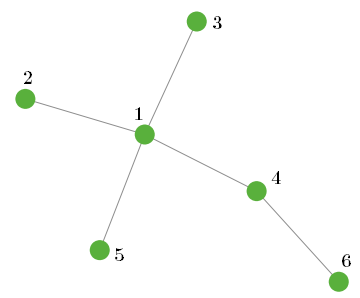
\includegraphics[width=0.5\linewidth]{../Figures/stability/Unefficientbutstablestar.png}
  \caption{\label{fig:stablestar} The resulting network after a simulation with the parameters from table \ref{tbl:stablestar} .}
\end{figure}
As we see this is not an efficient star, but the network is stable. The efficient network would be to delete the link $4,6$ and adding the link $1,6$. But since we only consider a link at a time this can not be done. To show this let $U_{i}$ denote the payoff of node $i$, the payoffs of the nodes are as described in eq (\ref{eq:payoffstablestar}).
\begin{eqnarray}
U_{1}=4\beta+\beta^2-4c\\
U_{2}=U_{3}=U_{5}=\beta+3\beta^2+\beta^3-c\\
U_{4}=2\beta+3\beta^2-2c\\
U_{6}=\beta+\beta^2+3\beta^3-c
\label{eq:payoffstablestar}
\end{eqnarray}
Node $6$ would benefit from adding the link $1,6$, but node 1 is not willing to do so because then he must pay an extra cost, and since $\beta^2>\beta-c$. Thus the network is stable but not efficient. 

\subparagraph{Star not possible with high $n$}
In the paper \cite{jackson2005survey} they come up with this proposition:
Consider the symmetric connections model in the case where $\beta-\beta^2<c<\beta$. As the number of nodes grows, the probability that a stable state (under the process where each link has an equal probability of being identified) is reached with the efficient network structure of a star goes to 0. But if a network reaches the efficient star structure, it is also pairwise stable, and will remain a star. 
We confirmed this when running multiple simulations, when we used few nodes the resulting network often became a star, but as the number of nodes increased the network rarely was a star. 

However, the structure of the networks are very similar to a scale-free network. There are many nodes with low node degree, and few with a high node degree.
One example of this is shown in figure \ref{fig:stablescalefree}, there are only ten nodes, but the network have the properties of a scale-free. Two nodes with degree of 4, and the rest have a degree of one or two.
\begin{figure}[h]
\centering
  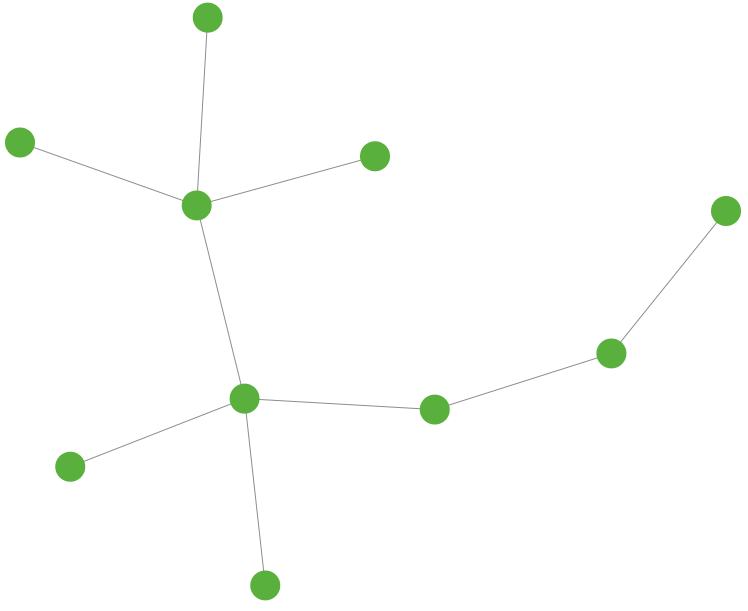
\includegraphics[width=0.5\linewidth]{../Figures/stability/Unefficientbutstabletwo.png}
  \caption{\label{fig:stablescalefree} The resulting network after a simulation with the parameters from table \ref{tbl:stablestar} and ten nodes.}
\end{figure}
\subparagraph{Bulk insurance}
As noted before it is not preferable to be the center node, due to the cost of all the direct links. If we consider the model with bulk insurance discount, this would lower the extra cost for the center node significantly. This could be used to increase the probability of reaching a star formation. 

Using the discount formula from the previous model, we end up with the equation (eq \ref{eq:discountstar}) to achieve a efficient and stable star topology. $i$ represents the node degree.
\begin{equation}
\beta-\beta^2<\frac{i_{l}}{i+1}< \beta
\label{eq:discountstar}
\end{equation}
An interesting property of the discount model is that the conditions for a efficient networks will change. Because
when the node degree increases, the insurance cost might reach the critical degree $g$, see (eq \ref{eq:criticaldiscount}). 
\begin{equation}
\frac{I_{l}}{g}<\beta-\beta^2
\label{eq:criticaldiscount}
\end{equation}
For this to be possible $g<n$, where $n$-represents the number of nodes in the network.
The stability condition have changed for a node with a critical degree, the stable and efficient condition for this node is, as shown earlier, to have a direct connection to every other node. Thus if we have a star-topology both the leaf nodes and the center nodes are stable, and the center node has been compensated for its role in the network.

Since the networks formed are similar to scale-free networks, we can calculate the probability of a node having degree $g$, see (eq \ref{eq:probabilitydegree}). $\gamma$ is the power law parameter, as described in Chapter \ref{chp:graphTheory}.
\begin{equation}
P(g)=g^{-\gamma}
\label{eq:probabilitydegree}
\end{equation}
When a node $i$ reaches the critical degree $g$ its optimal strategy is to connect to every node, since the payoff of direct connection is larger than any indirect connection. In general nodes prefer to connect to nodes with high connectivity \footnote{A node with high degree implies a node with high connectivity.}, and will thus prefer to connect to this node compared to nodes with a degree lower than $g$. In this way nodes will connect to the node who have a degree greater or equal to $g$, and remove the links to their low-degree nodes which they can instead reach through  $i$.
Lets consider a case with $n-$nodes, and two of these nodes, $i$ and $j$, have an equal degree larger than $g$. The rest of the nodes has a degree of one or zero. If there exists a node with degree zero, it would prefer to be connected to $i$ or $j$, and so will $i$ and $j$, so this will eventually happen.
If a node connected to $i$ are considering connecting to $j$, or visa versa, it will do so because $j$ can offer a higher connectivity than $i$. Now $j$ has a higher degree than $i$, and thus every node would prefer to connect to $j$ over $i$. This will eventually result in a star formation, with $j$ as the center node. 
From this we get the propositions:
\begin{proposition}
If the probability that there exists a node with a critical degree is very high, the resulting network will with high probability end up in a network where the average degree is close to the max-degree. 
\label{prop:clique}
\end{proposition}
\begin{proposition}
If the probability that there exists a node with critical degree, is such that only a few nodes will reach this degree, then the resulting network will be a star-topology. 
\label{prop:star}
\end{proposition} 

\subsection{Simulation}
To see if the propositions above where true, we created a simulator. The rules of the game are as follows.
Every round two random nodes, not neighbors, are selected, and asked if they would want to establish a link. The link establishment is a symmetric decision. If the link is added, we check if either of the nodes would prefer to delete some of their already existing links, this decision is asymmetric. This procedure is repeated as long as there are possible to add new links. 
The payoff function of each node is as described earlier( see (eg \ref{eq:connecetionGame})), except that the cost is now dependent on the degree of the node.
We know that if (eg \ref{eq:discountstar}) is satisfied for all $i$, then the efficient and stable state is a star. But whats of interest is when some nodes reaches the critical degree.
\subparagraph{Low critical node degree}
It is reasonable to believe that if the critical degree is low, the probability of the resulting network being a star will be high. But as we will see, this is not the case. If we consider the variables and their values shown in (table \ref{tbl:clique}), $n-$ is the number of nodes. We see that (eg \ref{eq:discountstar}) is satisfied until a node is considering establish its third direct link. At this point the node has reached the critical degree, and will strictly prefer to establish direct links. This will lead to even more nodes reaching the critical degree level, and the result is that almost every node connects to every one else. Two of the resulting simulating networks with these parameters can be seen in figure \ref{fig:discounthighdegree}. As we can see from the parameters in table \ref{tbl:clique}, the critical degree is reached when a node gets a degree of two. From degree two and up, $c<\beta-\beta^{2}$. The expected number of nodes with degree of two are $E(g=2)=10*2^{-2}=2.5$. This is when we assume that the network follow a power-law with $\gamma=2$.  This is considered as a high expected number. The same observations where seen in network with more nodes, from ten to forty.
\begin{table}[h]
\centering
\begin{tabular}{lc}
 \hline
  $
  n=10,
  \beta=0.7,
  \beta-\beta^2=0.21,
  I_{l}=0.6$\\
  \hline
\end{tabular}
\caption{The parameters used in the simulation in \ref{fig:stablestar} \label{tbl:clique}}
\end{table}

\begin{figure}[h]
\centering
\begin{subfigure}{.5\textwidth}
  \centering
  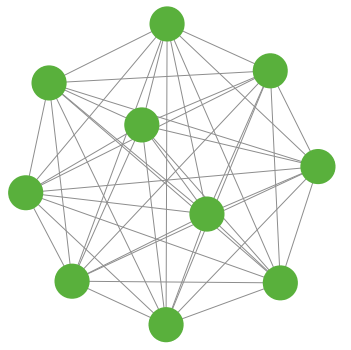
\includegraphics[width=0.4\linewidth]{../Figures/discount/cliquetennodes.png}
  \caption{\label{fig:discountclique} A clique consisting of ten nodes. }
\end{subfigure}
\quad
\begin{subfigure}{.46\textwidth}
  \centering
  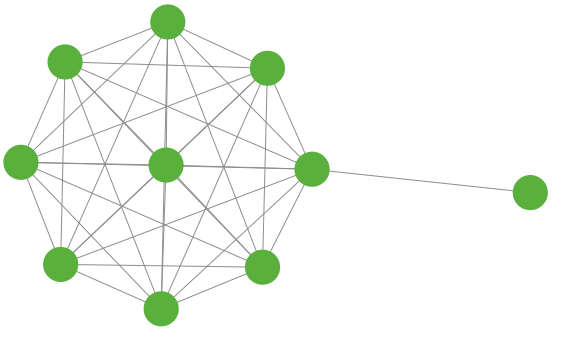
\includegraphics[width=0.8\linewidth]{../Figures/discount/baloontennodes.png}
  \caption{\label{fig:discountbaloon} A network with high average node degree, but not a clique.}
\end{subfigure}
\caption{\label{fig:discounthighdegree} Two different outcomes of the simulations with parameters from table \ref{tbl:clique}.}
\end{figure}

\subparagraph{High critical node degree}
To ensure that the network will form a star, we have to find parameters such that, equation (eq \ref{eq:discountstar}) is satisfied, and the probability of a node having a critical degree has to be relative low. In a network with ten nodes, the expected number of nodes with degree five in a network with ten nodes, is $E(g=5)=10*5^{-2}=0.4$. With the parameters from table \ref{tbl:discountstar}, these conditions are satisfied and the resulting network can be seen in figure \ref{fig:star:a}.
  
\begin{table}[h]
\centering
\begin{tabular}{lc}
 \hline
  $
  n=10,
  \beta=0.8,
  \beta-\beta^2=0.16,
  I_{l}=0.7$\\
  \hline
\end{tabular}
\caption{The parameters used in the simulation in \ref{fig:startennodes} \label{tbl:discountstar}}
\end{table}

\begin{figure}[h]
\centering
\begin{subfigure}{.9\textwidth}
  \centering
 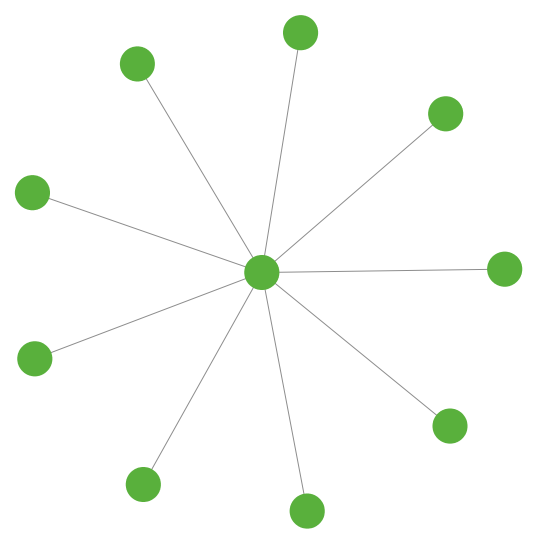
\includegraphics[width=0.4\linewidth]{../Figures/discount/startennodes.png}
  \caption{\label{fig:star:a} The result of simulating with the parameters in table \ref{tbl:discountstar}, a star with ten nodes}
\end{subfigure}
\quad
  
\begin{subfigure}{.9\textwidth}
  \centering
  \includegraphics[width=0.4\linewidth]{../Figures/discount/starmanynodes.png}
  \caption{\label{fig:star:b} A star network formed when running a simulation with forty-nodes, and parameters satisfying proposition \ref{prop:star}}
\end{subfigure}
\caption{\label{fig:star1} Two star-network, ten- and forty-nodes, both are the result of simulations with parameters satisfying proposition \ref{prop:star}.}
\end{figure}
These results where confirmed by running the simulation several times, and also by running several simulations with $n \geq 10 \text{ and } n\leq 40$. In every simulation the expected number of nodes with a critical degree was set to areas between $0.2 - 0.4$. And every time it resulted in a star-topology.

Another possibility for solving the problem with unfair costs, could be to use a shared-network cost instead. i.e. every node pays a cost equal to the total cost of the network divided on the number of nodes. 
Similar value distribution has been analyzed by Jackson and Wolinsky in \cite{jackson1996strategic}, and is called an egalitarian allocation rule, this rule guarantees that any efficient network is also pairwise stable. But this is unfortunately a very extreme rule.


\chapter{Model from Bohme}


Our model now includes a way of analyzing indirect connectivity among nodes. Inspired by the paper from \cite{danezis2006network} we are now expanding the model to look how network formation works when the nodes have a option to include uninsured nodes in their network. Although the paper tries to observe suseptibility to sybil attacks in peer-to-peer networks, their approach on network formation is related to our insurance network. They propose a network formation game consisting of "friends" and "strangers", which is similar to "insured" vs "non-insured" nodes. 
In a peer-to-peer network the peers selfishly tries to fulfill their communitaction needs, by establishing connections to friends or indirectly via strangers. This is similar to how companies selfishly choose to connect to other nodes with the goal of increasing their utility as much as possible. 

In \cite{danezis2006network} the formation game shows how nodes routes messages between each other. The special case here is that a node does not have enough links to directly connect to everyone. We change the game variables to fit to our model, and the setup for the game is as follows:

\begin{enumerate}

\item There are a set of $N nodes$ which are to be connected in a graph.
\item Each node, $n$ has a set for friends (insured nodes) $F_{n}$ which he want to connect to. The friendship is symmetric.
\item Each node also has a \textit{link budget}, $L_{n}$ which specifies the maximum number of links a node can establish directly to friends. It is also assumed that $L_{n}<F_{n}$. Additionally, if a link is established both nodes will decrease their link budget.
\item Given a graph of links between nodes the utility of each node is calculated using the negative sum of the length of the shortest path to all it friends. Negative sum yields higher utility as the different path lengths decreases.
\end{enumerate}

The goal is obviously to increase the utility. To accomplish this one has to communicate with friends using a minimum number of hoops. If $L_{n}=<F_{n}$ the game would have been a straightforward dominant strategy, where insured nodes only chose to connect to other insured nodes. Hence every node would receive the maximum utility. In the scenario of peer-to-peer network it is easy to understand that one cannot have direct links to every friend on a scale free network, e.g. the Internet, hence $L_{n}<F_{n}$ makes perfect sense. It is also reasonable to take the same assumption  for the insurance market, since one might not have the resources to insure every connection needed, i.e. the link budget $I_{n} < F_{n}$. Hence the nodes might take the risk of connection to non-insured nodes, since the cost of connecting to this node is free.

The graph is created by a pseudo-random selection of a possible link between two nodes. If the utility increases or is stable for both, the link is created and each node decreases their link budget by one.

 
\cite{danezis2006network} proposes two random games which interpret that nodes might have to take the risk of connecting to non-insured nodes.
\begin{enumerate}
\item Random model: Every node in the network initiate a set for friendships with other nodes, denoted $F$. All nodes have the same link budget $L<F$. 
\item Unbalanced Random Mode. The same friendship graph as in the random model is created. However one of the nodes have a significantly larger link budget $(L_{0} > 2 F)$
\end{enumerate}

The first model does not result in any Nash equilibrium, it is believed that every node is eager to use their whole link budget in order to create direct connections to as many insured nodes as possible. In order to reach the rest of the insured nodes, they rely on indirect connectivity via the established connections.

The unbalanced model results in a scenario where the insured nodes still wishes to connect to other insured nodes. The reason for this is claimed to be that the average shortest path in a scale-free graph is $O(log N)$, and the probability that another node, insured or not insured, is closer to to a node is roughly the same. Which means that on average an insured node will benefit from connecting to other insured nodes. 
However, if the link budget only allows each node to only establish 1 link (except the one with a large budget), it will emerge a Nash equilibrium which is star with the rich node in the center. If the rich node is a insured node, all the other insured nodes will connect to this node. 

Maa tilpasse konklusjonene her bedre..









